%--------------------------------------------------------------------------------------------------------------------------------------------------------------------------------
%  Template na zaverecne diplomove alebo bakalarske prace 
%  Autor: Jakub Uhrik
%  site: http://jakuub.uhrikovci.sk/
%  licencia: robte s tym co chcete, len mi nenadavajte, pouzivate to na vlastne riziko :)
%  zdroje: misofov template pre zaverecne prace
%  Zakladne subory plus funkcia:
%    -  main.tex                            - zakladny subor z ktoreho sa na vsetko odkazuje
%    -  config.tex                          - subor, v ktorom nastavite zakladne veci ako meno prace....
%    -  content/structure/                  - tu sa nachadzaju subory, v ktorych su zakladne casti struktury prace ako titulka, abstrakt ...
%    -  content/structure/abstract.tex      - tu vyplnite abstrakty
%    -  content/structure/obalka.tex        - tu nic nevyplnate, subor sa vyplni udajmi z config.tex
%    -  content/structure/prehlasenie.tex   - tu vyplnite prehlasenie, ktore ale pokial viem teraz nie je povinne
%    -  content/structure/thanks.tex        - tu je podakovanie, mozete sa inspirovat mojim alebo vytvorit originalne
%    -  content/structure/titulka.tex       - tu nic nevyplnate, subor sa vyplni udajmi z config.tex
%    -  content/structure/zadanie.tex       - tu nastavite, ci mate aj anglicke zadanie, alebo len slovenske a najdete pokyny ako a co...
%    -  content/chapters/chapters.tex       - tu musite includovat vsetky kapitoly. Neda sa to jednoducho robit automaticky
%    -  content/chapters/intro.tex          - tu napisete intro
%    -  content/chapters/zaver.tex          - a tu zaver
%    -  content/chapters/01.tex             - tu je prva kapitola, je vynimocna, lebo sa v nej meni pagestyle. V kazdej dalsej uz nie je nic vynimocne....
%    -  content/chapters/02.tex             - kazda dalsia bezna kapitola, toto je len tempalte
%
%  V pripade, ze pouzivate make, pomocou obycajneho prikazu "make" sa vam vytvori pdf subor s pracou. Potrebujete na to ale aplikacie:
%    - pdfcslatex
%    - bibtex
%  Makefile obsahuje aj dalsie moznosti, ale tie su teraz irelevantne...
%
%  V pripade, ze by ste chceli pouzit git, je tu vytvoreny nejaky .gitignor, v ktorom su ignorovane subory nepotrebne pre beh tohoto tu, 
%  cize sa budu zalohovat len podstatne veci
%
%  To by malo byt snad vsetko, prajem prijemne pouzivanie. 
%--------------------------------------------------------------------------------------------------------------------------------------------------------------------------------

\documentclass[oneside, 12pt]{book}
\usepackage[slovak]{babel}
\usepackage{epsfig}
\usepackage{color}
\usepackage{url}
\usepackage[utf8]{inputenc}
\usepackage[T1]{fontenc}
\usepackage{lmodern}

%------------------------------------------------------------------------------------------------------
% inportujeme subor s nastaveniami vsetkych zakladnych veci
%------------------------------------------------------------------------------------------------------

%------------------------------------------------------------------------------------------------------
% pekne pokope definujeme potrebne udaje
%------------------------------------------------------------------------------------------------------
\def\mftitle{Názov diplomovej/bakalárskej práce}          % nazov diplomovky/bakalarky
\def\mfthesistype{Bakalárska/Diplomová práca}             % typ prace
\def\mfkeywords{key words, key key wordddd :)... }        % proste klucove slova idealne oddelene ciarkou
\def\mfkeywordsen{key words, key key wordddd :)... }      % klucove slova v anglictine EN
\def\mfkeywordssk{key words, key key wordddd :)... }      % klucove slova v slovencine SK
\def\mfauthor{Meno Priezvysko}                            % vase meno a priezvysko
\def\mfadvisor{Školitel}                                  % cele meno skolitela
\def\mfplacedate{Bratislava, 2012}                        % mesto a rok
\def\mfdate{2012}                                         % Rok
\def\mfuniversity{Univerzita Komenského, Bratislava}      % Univerzita
\def\mffakulta{Fakulta Matematiky, Fyziky a Informatiky}  % Katedra
\def\mffakultafull{Fakulta Matematiky, Fyziky a Informatiky Univerzity Komenského v Bratislave}  
                                                          % Katedra v plnom zneni aj s univerzitou
\def\mfprogram{Informatika}                               % studijny program
\def\mfodbor{2508 Informatika}                            % studijny odbor
\def\mfpracovisko{Katedra Informatiky}                    % skoliace pracovisko



%------------------------------------------------------------------------------------------------------
% odsadenie textu z bokov, zhora a z dola
%------------------------------------------------------------------------------------------------------
\usepackage[a4paper,vmargin={25mm,25mm},hmargin={35mm,20mm}]{geometry} 
\usepackage{minted}
\hyphenpenalty=10000
\tolerance=10000

\usepackage[ps2pdf,
	bookmarks=true,
	bookmarksnumbered=false, 	% true means bookmarks in
								% left window are numbered
	bookmarksopen=false,
								% true means only level 1
								% are displayed.
	colorlinks=true,
	pdftitle={\mftitle},
	pdfauthor={\mfauthor},
	pdfsubject={\mfthesistype},
	pdfkeywords={\mfkeywords},
	pdfproducer={\mffakultafull},
	linkcolor=webblue]{hyperref}
\definecolor{webgreen}{rgb}{0, 0.5, 0} % less intense green
\definecolor{webblue}{rgb}{0, 0, 0.5} % less intense blue
\definecolor{webred}{rgb}{0.5, 0, 0}
\definecolor{grey}{rgb}{0.5, 0.5, 0.5}
\definecolor{white}{rgb}{0.95, 0.95, 0.95}
\definecolor{black}{rgb}{0, 0, 0}
%------------------------------------------------------------------------------------------------------
% less intense red
%------------------------------------------------------------------------------------------------------

\usepackage[final]{pdfpages}

 
%------------------------------------------------------------------------------------------------------
% riadkovanie jeden a pol
%------------------------------------------------------------------------------------------------------
\renewcommand\baselinestretch{1.3} 

\author{\mfauthor}
\title{\mftitle}

\begin{document}

%------------------------------------------------------------------------------------------------------
% vlozime strukturu, vyplnte ju priamov suboroch, treba len pomenit texty
%------------------------------------------------------------------------------------------------------
%------------------------------------------------------------------------------------------------------
%  toto je subor obalky vasej prace. 
%  s tymto by ste asi ani nemali nic robit pouziju sa prednastavene veci z hlavneho suboru
%------------------------------------------------------------------------------------------------------
\frontmatter

\thispagestyle{empty}

\noindent
\begin{center}
\begin{minipage}{0.8\textwidth}
\centerline{\renewcommand\baselinestretch{1.3} \LARGE\sc\mfuniversity}
\centerline{\sc\mffakulta}
\end{minipage}
\end{center}

\vfill
\begin{center}
\begin{minipage}{1\textwidth}
\bigskip\bigskip
\begin{center}
\linespread{1}\LARGE\sc\mftitle
\end{center}
\smallskip
\centerline{\mfthesistype}
\bigskip
\bigskip
\bigskip\bigskip
\end{minipage}
\end{center}
\vfill
{\bf\mfdate\\
\indent\mfauthor}
\eject 



%------------------------------------------------------------------------------------------------------
%  toto je titulna stranka, vsetky veci ste nastavili v config.tex
%------------------------------------------------------------------------------------------------------
\thispagestyle{empty}

\noindent
\begin{center}
\begin{minipage}{0.8\textwidth}
\centerline{\LARGE\sc\mfuniversity}
\centerline{\sc\mffakulta}
\end{minipage}
\end{center}

\vfill
\begin{center}
\begin{minipage}{1\textwidth}
\bigskip\bigskip
\begin{center}
\linespread{1}\LARGE\sc\mftitle
\end{center}
\smallskip
\centerline{\mfthesistype}
\bigskip
\bigskip
\bigskip\bigskip
\end{minipage}
\end{center}
\vfill
\begin{minipage}{0.8\textwidth}
\begin{tabular}{l l}
Študijný program:& \mfprogram \\
Študijný odbor:& \mfodbor \\
Školiace pracovisko:& \mfpracovisko\\
Školiteľ:&   \mfadvisor \\
\end{tabular}
\end{minipage}
\begin{center}
\end{center}
\vfill
{\bf\mfplacedate\\
\indent\mfauthor}
\eject 



%------------------------------------------------------------------------------------------------------
%  pdf zadania dajte do zlozky images v subore zadanie.pdf tak ako vidite v prikaze. 
%  ak zadavate aj anglicke zadanie, odkomentujte(odstrante percento zo zaciatku) 
%  druhy riadok a podla neho pridajte adekvatne pdf
%------------------------------------------------------------------------------------------------------

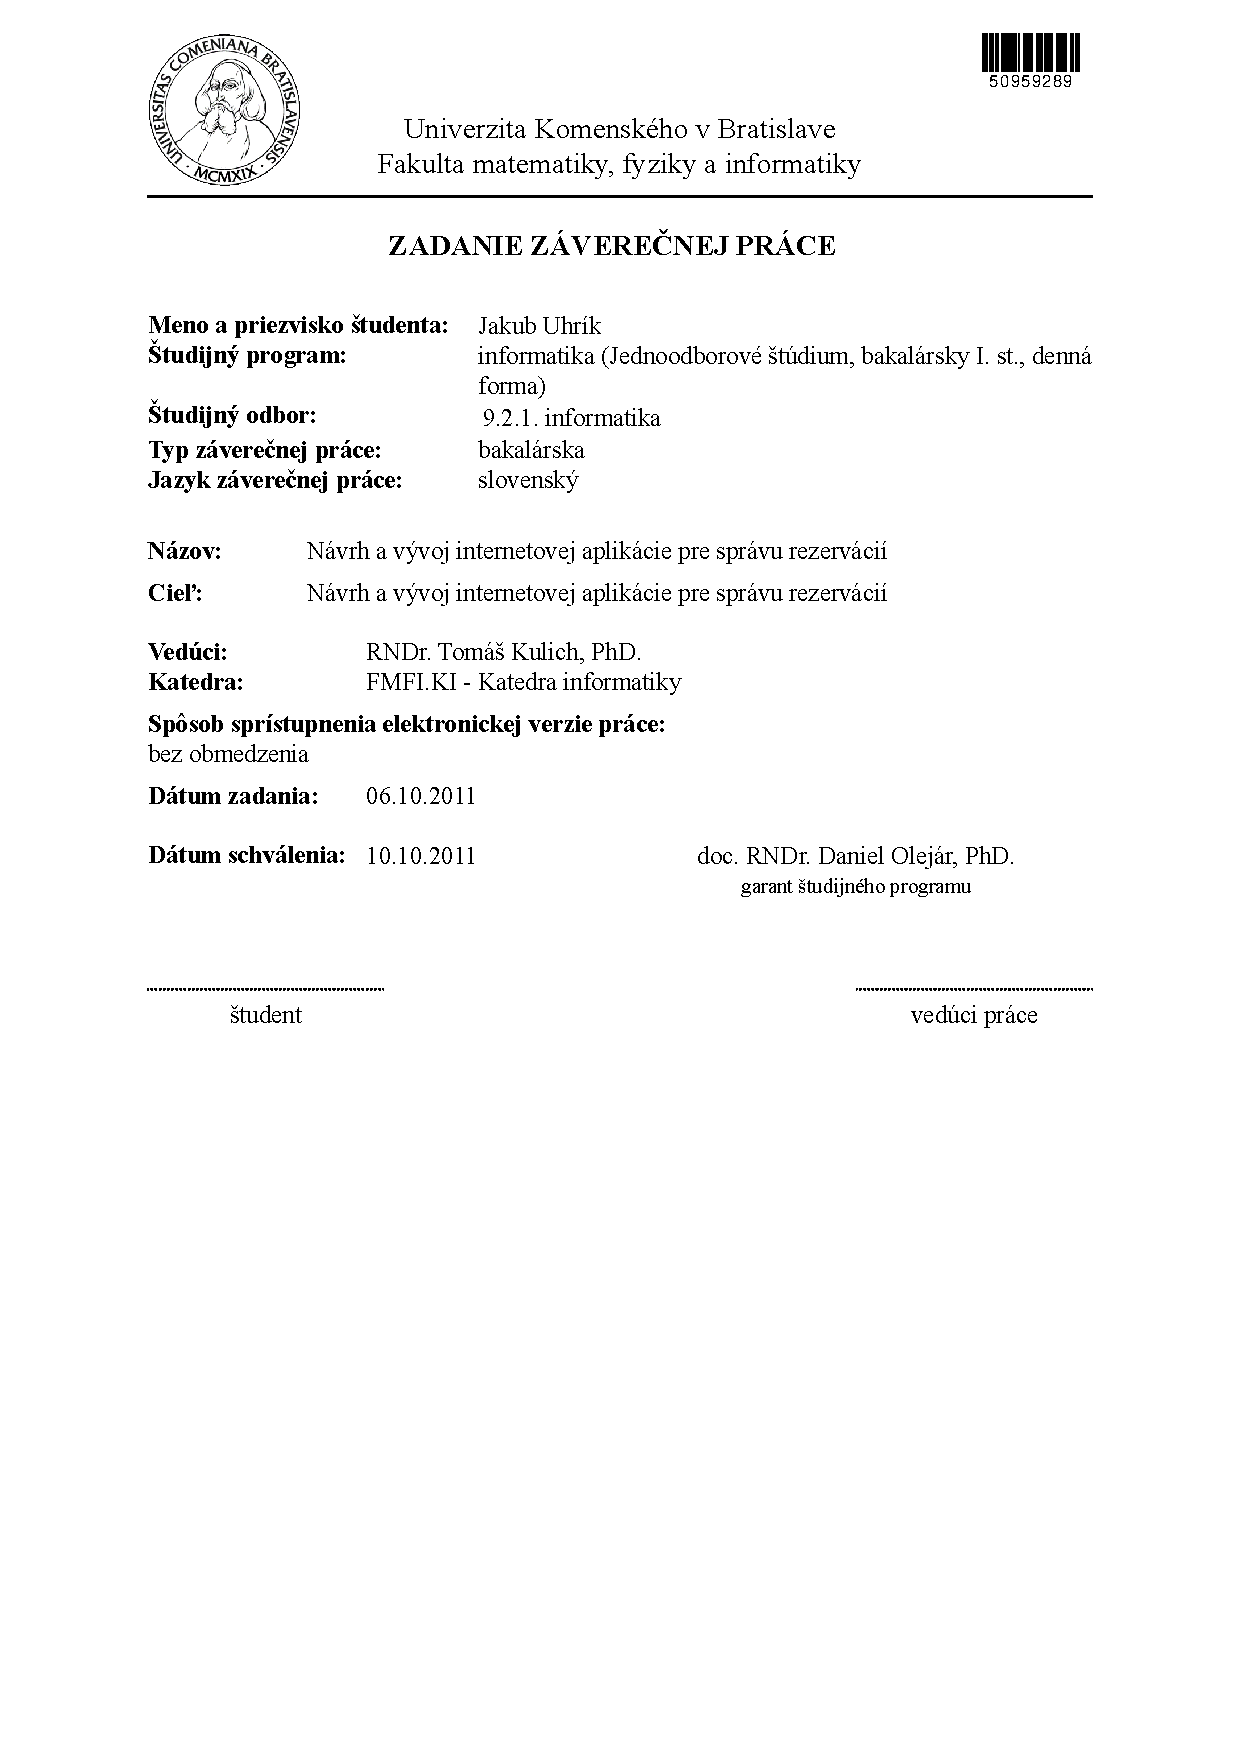
\includepdf{images/zadanie-en.pdf}
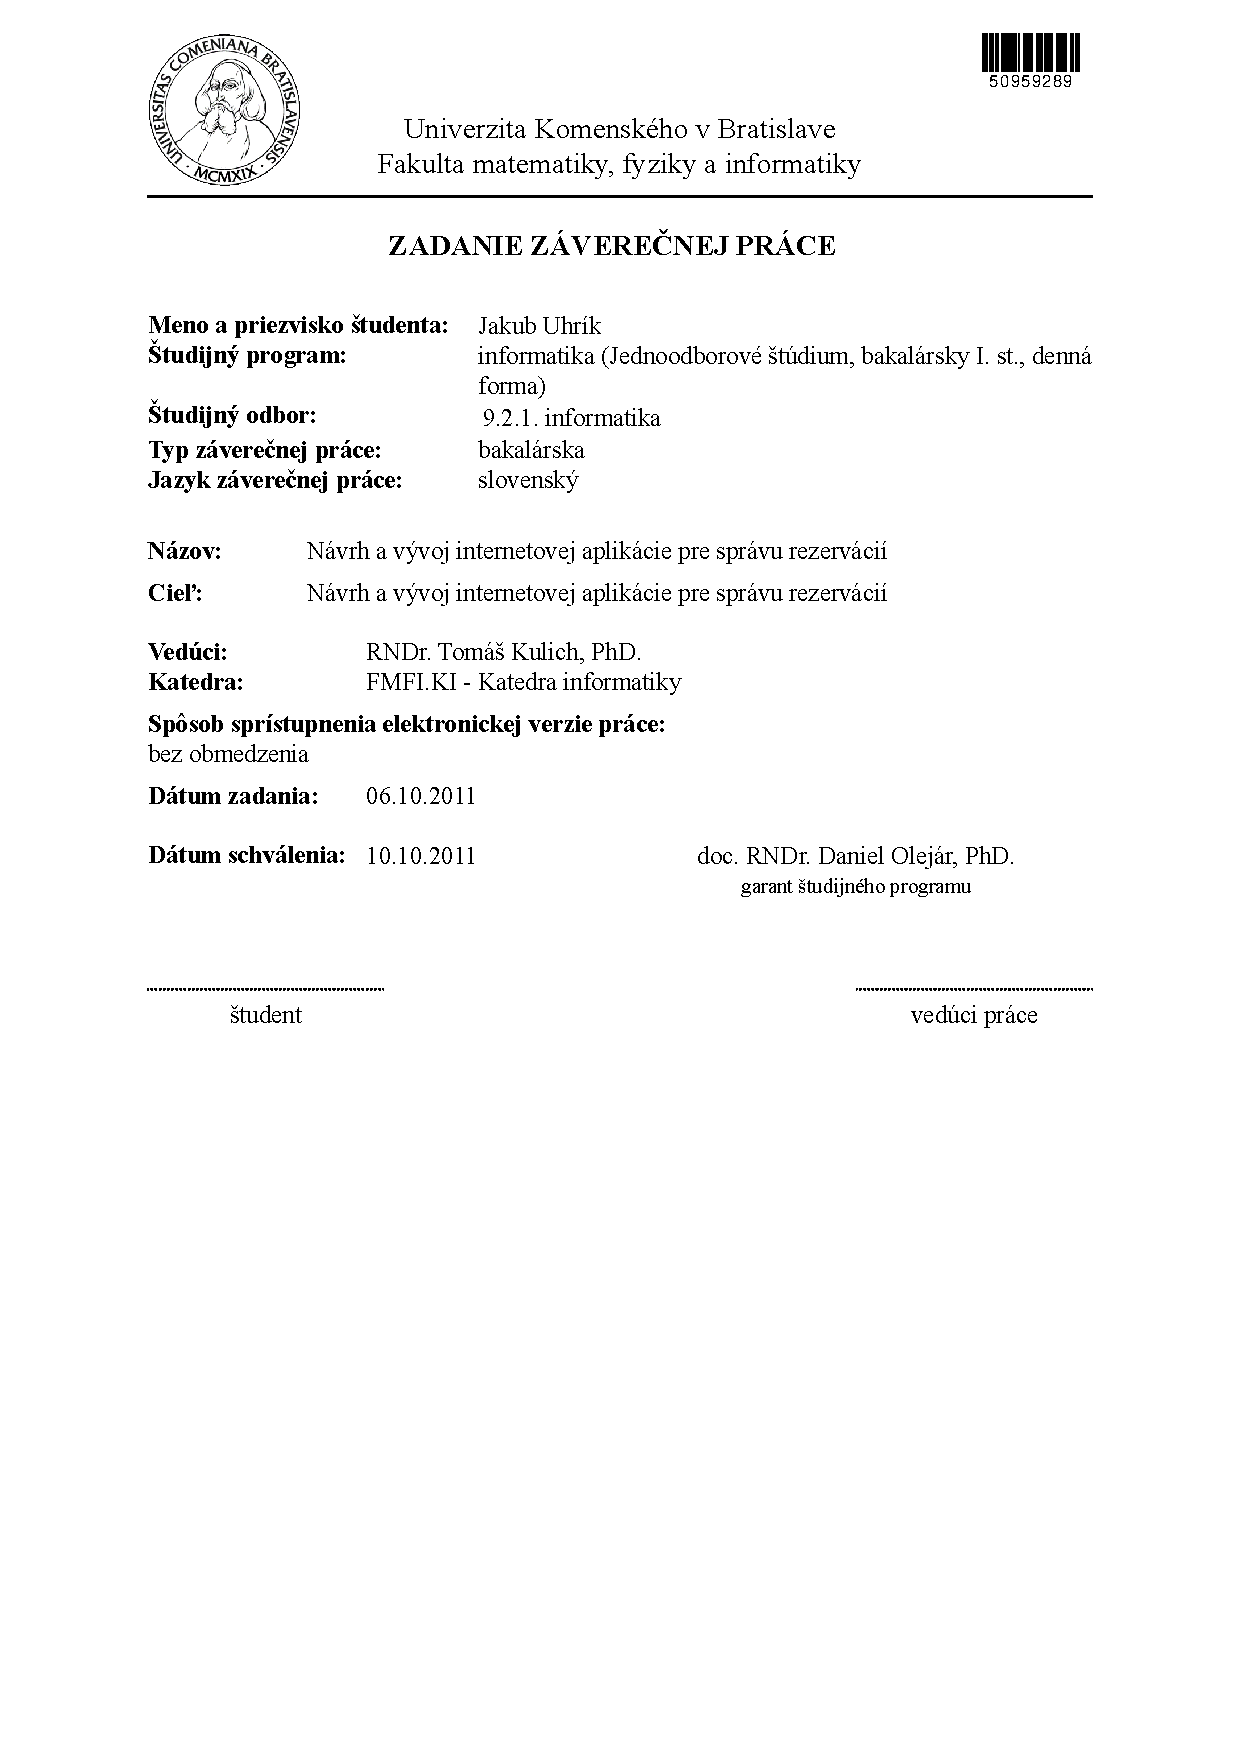
\includepdf{images/zadanie.pdf}
% 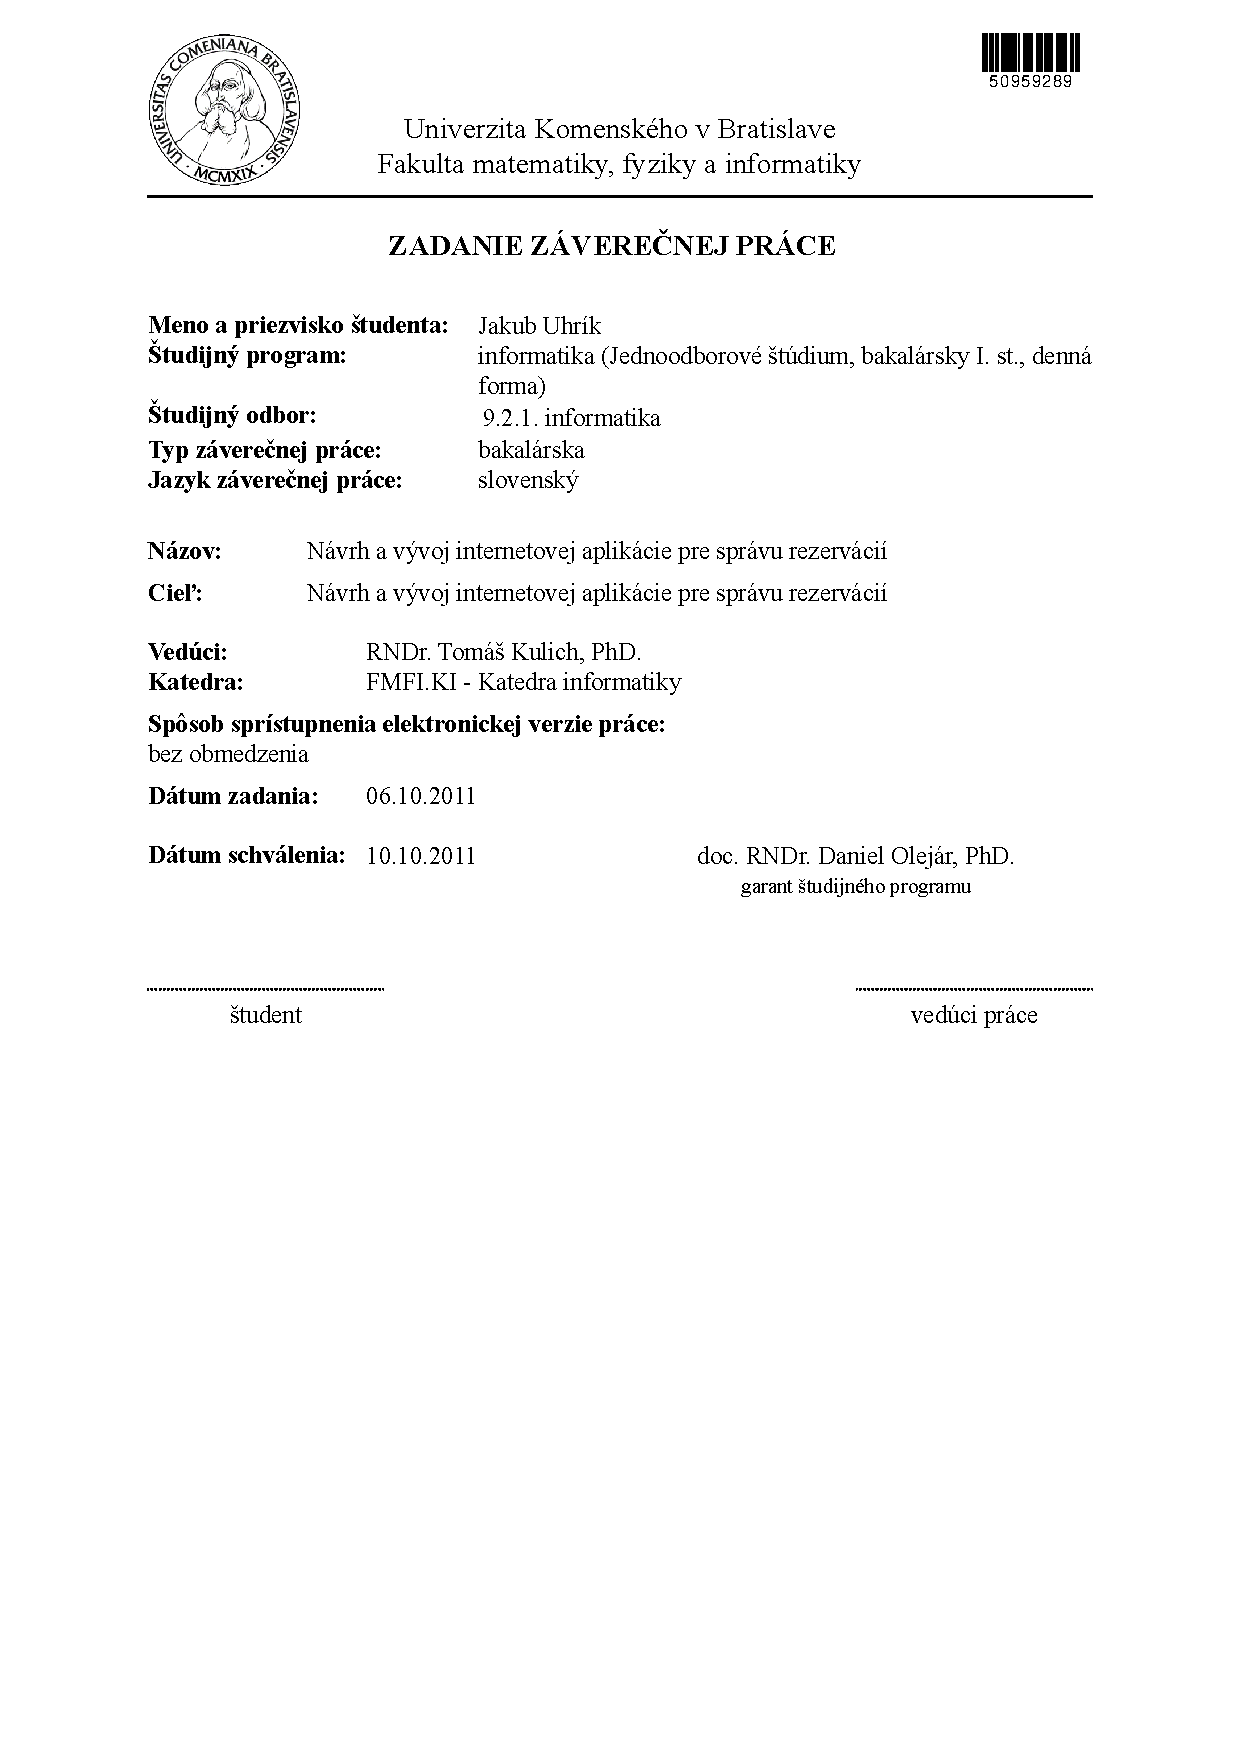
\includepdf{images/zadanie-en.pdf}



%------------------------------------------------------------------------------------------------------
% ked treba, da sa vlozit cestne prehlasenie...
%------------------------------------------------------------------------------------------------------
%%------------------------------------------------------------------------------------------------------
% prehlasenie, ze ste to poctivo sami vypracovali...
%------------------------------------------------------------------------------------------------------
{~}\vspace{12cm}

\noindent
\begin{minipage}{0.25\textwidth}~\end{minipage}
\begin{minipage}{0.68\textwidth}
%------------------------------------------------------------------------------------------------------
% sem kludne pridajte vase originalne cestne vyhlasenie, ale mozete sa inspirovat mojim
%------------------------------------------------------------------------------------------------------
I hereby declare that this thesis represents my own work and effort. Where other sourcesof information have been used, they have been acknowledged.

\bigskip\bigskip

\hfill\hbox to 6cm{\dotfill}
\end{minipage}
\vfill\eject 



%------------------------------------------------------------------------------------------------------
% Podakovanie. Proste subor s podakovanim. Napiste sem komu dakujete, mozete sa inspirovat mojim
%------------------------------------------------------------------------------------------------------
{~}\vspace{12cm}

\noindent
\begin{minipage}{0.25\textwidth}~\end{minipage}
\begin{center}
\begin{minipage}{1\textwidth}
%------------------------------------------------------------------------------------------------------
%  sem pridajte svoj originalny text, alebo len prepiste \mfadvisor za vysklonovane meno vaseho veduceho
%------------------------------------------------------------------------------------------------------

Ďakujem vedúcemu bakalárskej práce \mfadvisor za cenné rady 
a pripomienky, rodine a blízkym priateľom za pomoc a morálnu podporu.

\end{minipage}
\end{center}
\hfill\mfauthor
\vfill\eject 



%------------------------------------------------------------------------------------------------------
% Toto je subor s abstraktom. Pridajte sem vas/tvoj abstrakt v slovencine a/alebo anglictine
% Ak chcete len jeden abstrakt, vymazte vsetko medzi komentarmi "jazyk zaciatok" a "jazy koniec"
%------------------------------------------------------------------------------------------------------

%------------------------------------------------------------------------------------------------------
% EN zaciatok
%------------------------------------------------------------------------------------------------------
\noindent
\begin{center}
\begin{minipage}{1\textwidth}
\centerline{\large Abstract}
Abstract in english.
%------------------------------------------------------------------------------------------------------
% sem pridajte abstrakt v anglictine
%------------------------------------------------------------------------------------------------------
\\ \\ 
{\bf Key words:} \mfkeywordsen
\end{minipage}
\end{center}
\eject % EOP v
%------------------------------------------------------------------------------------------------------
% EN konie
%------------------------------------------------------------------------------------------------------

%------------------------------------------------------------------------------------------------------
% SK zaciatok
%------------------------------------------------------------------------------------------------------
\noindent
\begin{center}
\begin{minipage}{1\textwidth}
\centerline{\large Abstrakt}
%------------------------------------------------------------------------------------------------------
% sem pridajte abstrakt v slovencine
%------------------------------------------------------------------------------------------------------
Abstrakt v slovencine.
\\ \\ 
{\bf Kľúčové slová:} \mfkeywordssk
\end{minipage}
\end{center}
\eject % EOP v
%------------------------------------------------------------------------------------------------------
% SK konie
%------------------------------------------------------------------------------------------------------



%------------------------------------------------------------------------------------------------------
% obsah
%------------------------------------------------------------------------------------------------------
\tableofcontents

%------------------------------------------------------------------------------------------------------
% zoznam obrazkov
%------------------------------------------------------------------------------------------------------
\listoffigures

\mainmatter

%------------------------------------------------------------------------------------------------------
% page stype plain pre ciste strany bez cisiel stran pre uvod
%------------------------------------------------------------------------------------------------------
\pagestyle{plain}

%------------------------------------------------------------------------------------------------------
% a teraz includneme vsetky kapitoly, realne je to len subor, v ktorom sa incuduju kapitoly postupne
%------------------------------------------------------------------------------------------------------
\pagestyle{plain}
\input content/chapters/intro.tex
\pagestyle{headings}
\input content/chapters/motivation.tex
\input content/chapters/databinding.tex
\input content/chapters/existing.tex
\input content/chapters/our.tex
\input content/chapters/performance.tex
\input content/chapters/benchmarks.tex
\pagestyle{plain}
\input content/chapters/conclusion.tex


\backmatter

%------------------------------------------------------------------------------------
% vyprodukujeme bibliografiu zo suboru literatura.bib
%------------------------------------------------------------------------------------
\nocite{*}
\bibliographystyle{alpha}
\bibliography{literatura.bib}

\addcontentsline{toc}{chapter}{Literatúra}


\end{document}
 
